\documentclass[10pt,a4paper]{article}
\usepackage[margin=2.1cm]{geometry}
\usepackage[T1]{fontenc}
\usepackage{lmodern}
\usepackage{amsmath,amssymb}
\usepackage{graphicx}
\usepackage{booktabs}
\usepackage{xcolor}
\usepackage{listings}
\usepackage{enumitem}
\usepackage[hidelinks]{hyperref}
\usepackage{caption}
\captionsetup{font=small,labelfont=bf}
\setlist{itemsep=2pt,topsep=3pt}
\definecolor{boxbg}{HTML}{EEF4FC}
\definecolor{codebg}{HTML}{F6F6F4}
\lstset{language=Python,basicstyle=\ttfamily\footnotesize,backgroundcolor=\color{codebg},
        frame=none,columns=fullflexible,keepspaces=true,showstringspaces=false,
        xleftmargin=4pt,aboveskip=4pt,belowskip=4pt}

\title{\vspace{-1.2cm}Choosing Hamiltonians for \texttt{EqualNumberOfBitstrings.py}\\[2pt]
\large a broad range of ground-state densities and initial overlaps}
\date{14 October 2026}
\author{}

\begin{document}
\maketitle
\vspace{-1.4cm}

\noindent\colorbox{boxbg}{\parbox{\dimexpr\linewidth-2\fboxsep}{%
\textbf{Recommendation in short}
\begin{enumerate}[leftmargin=1.4em]
\item \textbf{Tilt the field} instead of choosing between $B_z$ and $B_x$: draw an angle
  $\theta\sim U(0^\circ,90^\circ)$ from the $z$ axis and a strength
  $|B| = b\,|J|\max(1,\Delta)$ with $b$ log-uniform in $[0.1,10]$; set
  $B_x=|B|\sin\theta$, $B_z=|B|\cos\theta$. Keep $J\sim U(-1,1)$.
\item \textbf{Use} $\Delta\in\{0,\,0.5,\,1,\,2,\,5,\,10\}$. Drop $\Delta=100$: almost every such
  cell is removed by the gap or trivial-state filter. Add 2 and 5, which give the intermediate densities.
\item \textbf{Select for density}, do not just sample: draw candidates from 1.\ and keep
  2 per density bin of width 0.1, for every $(N,\text{dimension},\Delta)$
  (\texttt{select\_hamiltonians.py}). This gives 20 Hamiltonians per group, spread evenly from
  density $<0.1$ to $>0.9$ at \emph{every} $N$, and takes 30\,s on a laptop.
\item \textbf{Initial overlaps:} with these Hamiltonians, the uniform draw from the
  support already spans $10^{-11}$--$10^{-2}$. If large overlaps matter, draw the
  initial states stratified in $\log_{10}$ overlap. This raises the share above $10^{-2}$ from 6\% to 15\%.
\end{enumerate}}}

\section*{1\quad Why the two current draws do not cover the range}
The study's Hamiltonian is
$H = J\sum_{\langle ij\rangle}(X_iX_j+Y_iY_j+\Delta Z_iZ_j)-\sum_i(B_xX_i+B_zZ_i)$ with
$J,B\sim U(-1,1)$ and $\Delta\in\{0,0.5,1,10,100\}$. The density counts basis states with
$|\psi_i|>10^{-3}$. Cells with gap $<10^{-4}$ or top weight $\ge 1-10^{-10}$ are dropped.
I drew 20 Hamiltonians per $(N,\text{dim},\Delta)$ exactly as \texttt{enumerate\_cells} does
(Fig.~\ref{fig:density}, top two rows).

\begin{description}[leftmargin=0pt,style=unboxed]
\item[Longitudinal ($B_x=0$).] $H$ conserves the total magnetisation, so the ground state
  lives in a single $M_z$ sector. Its density can therefore never exceed
  $\binom{N}{N/2}/2^N$, which is $0.31$ at $N=6$ and $0.23$ at $N=12$. On top of that, 59\% of the
  cells are dropped. For $J<0$, $\Delta\ge1$ the ferromagnet is a single basis state. For large $\Delta$
  the two N\'eel states are split only at high order in $1/\Delta$.
\item[Transversal ($B_z=0$).] The symmetry is broken and the densities move up: 40\% of all cells
  are above $0.9$. Low densities need an ordered state ($\Delta\gtrsim 10$), but there a
  transverse field splits the two ordered states only at high order (growing with $N$). So the gap closes and
  the filter removes them: 46\% of the $\Delta=10$ and 89\% of the $\Delta=100$ cells.
  Only 2\% of the cells end up below $0.1$. This is what the shards in
  \texttt{bitstring\_shards\_heisenberg\_tv} show as well (201 of 424 kept cells above $0.9$).
\end{description}

\begin{figure}[h]
\centering
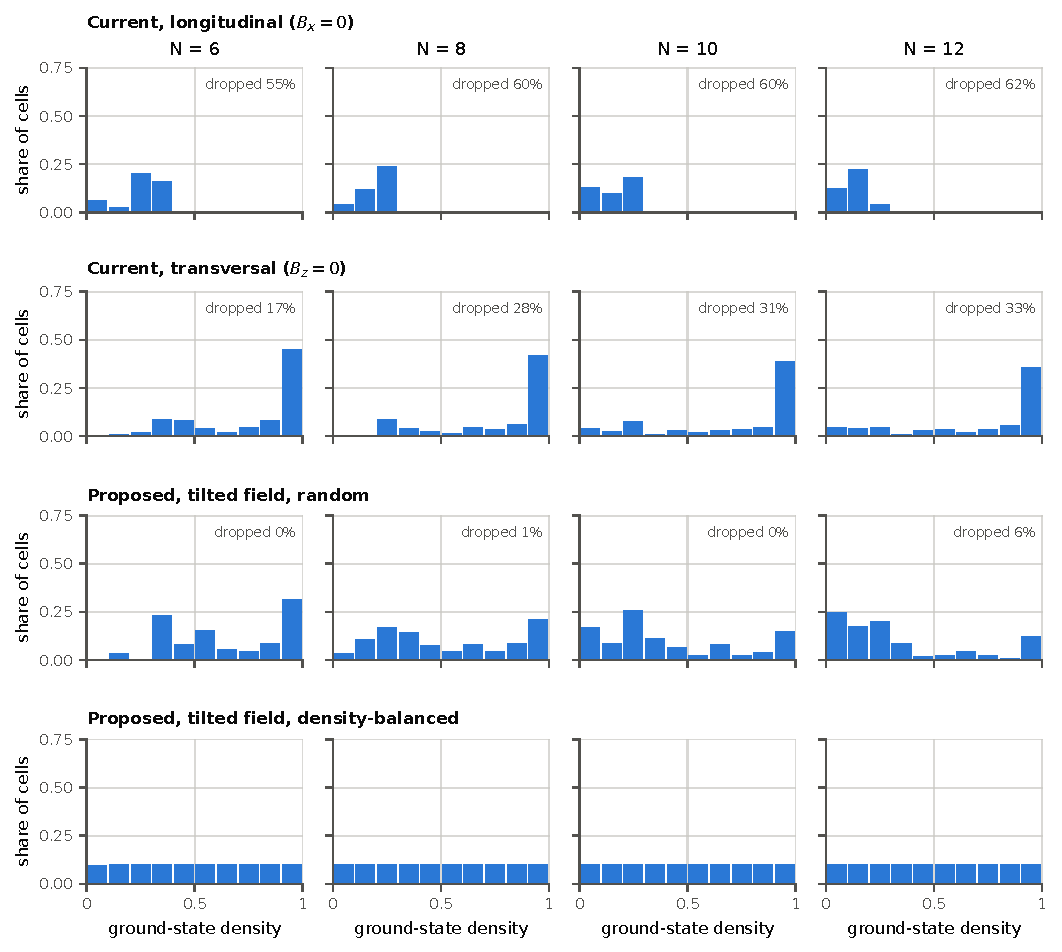
\includegraphics[width=\linewidth]{figures/density_comparison.pdf}
\caption{Ground-state densities of the cells that survive the gap and trivial filters. Bars are
shares of all drawn cells, so a row sums to the kept fraction. Each row is one way of drawing
the Hamiltonians: 20 per $(N,\text{dim},\Delta)$, both geometries pooled. Only the
density-balanced selection is flat at every $N$.}
\label{fig:density}
\end{figure}

\section*{2\quad What sets the density}
Figure~\ref{fig:mechanism} maps the density at $N=12$ over the two field parameters, from a scan of
11\,520 Hamiltonians ($N=6$--$12$, 1D and 2D, nine $\Delta$, both signs of $J$, ten field
strengths, eight angles; \texttt{scan\_grid.py}).
\begin{itemize}[leftmargin=1.2em]
\item \textbf{Strong field ($b\gg1$):} the ground state approaches the product state along
  the field. Its amplitudes are $\cos^{N-k}(\theta/2)\sin^k(\theta/2)$, so the angle alone sets the
  density: at $N=12$ it is $0.02,\,0.07,\,0.19,\,0.61,\,0.98$ for $\theta=5^\circ,15^\circ,30^\circ,45^\circ,60^\circ$.
  The gap is of order $|B|$, so all of these cells survive. This is the clean knob for the
  whole range.
\item \textbf{Weak field, $J>0$, $\Delta>1$:} N\'eel-like ground states with densities of a few
  per cent that survive the gap filter up to $\Delta\approx10$. These give the low end without
  being product states. At $\Delta=100$ they are lost (the gap is below $10^{-4}$).
\item \textbf{Weak field, $J<0$:} for $\Delta\ge1$ the ferromagnetic doublet is degenerate (pure
  $B_x$) or a single basis state (pure $B_z$). Any tilt between the two lifts both problems,
  which is why the tilted draw keeps 98--99\% of the cells.
\item The field has to compete with the largest coupling, $|J|\max(1,\Delta)$, and
  not with $|J|$ alone. Otherwise the high densities are out of reach at $\Delta=10$ on the 2D
  lattices. Hence the factor $\max(1,\Delta)$ in the recommended field strength.
\item At $\Delta=1$ the model is SU(2) symmetric. The field angle only rotates the basis, so
  for weak fields the density does not depend on $\theta$ (the singlet is rotation invariant).
\end{itemize}

\begin{figure}[h]
\centering
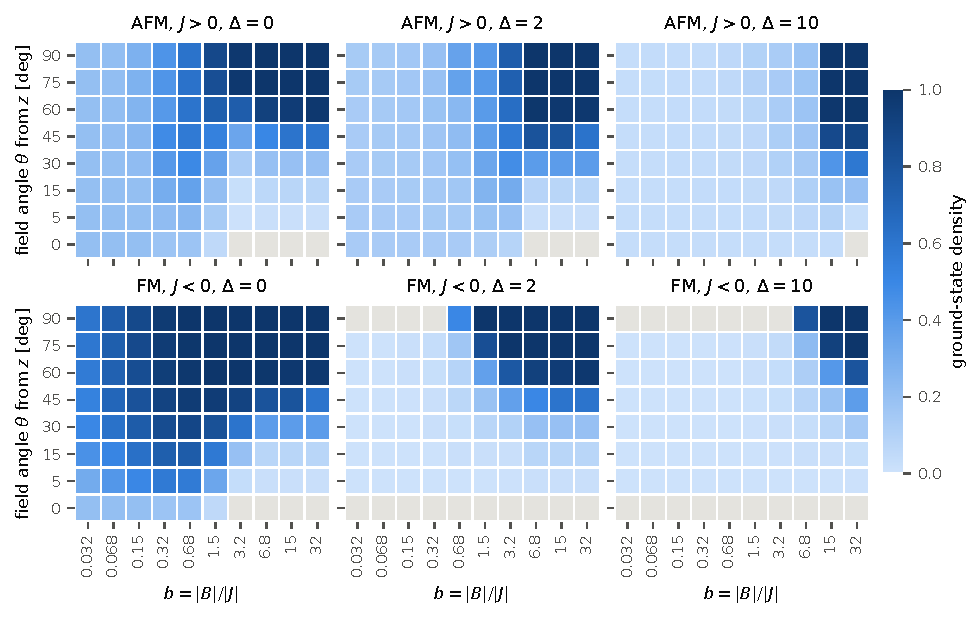
\includegraphics[width=\linewidth]{figures/mechanism.pdf}
\caption{Ground-state density at $N=12$ (1D) over field strength $b=|B|/|J|$ and angle
$\theta$ from the $z$ axis ($0^\circ$: longitudinal, $90^\circ$: transversal). Grey cells are
removed by the study's filters. The current study only uses the bottom row ($\theta=0$) or the
top row ($\theta=90^\circ$) of each panel.}
\label{fig:mechanism}
\end{figure}

\section*{3\quad Recommended parameters}
\paragraph{Random tilted field.} This is the minimal change to \texttt{enumerate\_cells}. Keep $J_1$ the first draw,
so that the longer-range couplings stay where they are:
\begin{lstlisting}
J_1, log_b, theta = rng.uniform(-1, 1), rng.uniform(-1, 1), rng.uniform(0, np.pi / 2)
...
B = 10 ** log_b * abs(J_1) * max(1.0, delta)     # per cell, since it depends on delta
Bx, Bz = np.round(B * np.sin(theta), 6), np.round(B * np.cos(theta), 6)
\end{lstlisting}
This keeps 98\% of the cells and spans $<0.1$ to $>0.9$ for $N\ge8$, but the distribution is still uneven
(Fig.~\ref{fig:density}, third row). At $N=6$ no cell falls below $0.1$, and at
$N=12$ few fall between $0.4$ and $0.9$. That is a consequence of the fixed threshold
$|\psi_i|>10^{-3}$: a flat state has amplitude $2^{-N/2}$, so the same ground state counts
differently at different $N$.

\paragraph{Density-balanced selection (recommended).} \texttt{select\_hamiltonians.py} draws
from the scheme above and keeps the first two Hamiltonians that land in each density bin
$[0,0.1),\dots,[0.9,1]$ and pass the study's filters. It does this for each $N\in\{6,8,10,12\}$, both geometries
and each $\Delta$. It filled 959 of the 960 slots from 32\,777 candidates in 32\,s. The one gap is
the lowest bin at $N=6$, 2D, $\Delta=0$, where a density below $0.1$ means at most six of 64
states. The resulting table (\texttt{data/selected\_hamiltonians.csv}) replaces the draw in
\texttt{enumerate\_cells}:
\noindent\begin{minipage}{\linewidth}
\begin{lstlisting}
table = pd.read_csv("StudyOfHamiltonians/data/selected_hamiltonians.csv")
return [Cell(int(r.hamiltonian_index), int(r.num_sites), int(r.dimension), float(r.delta),
             (float(r.J),), float(r.Bx), float(r.By), float(r.Bz), 1)
        for r in table.itertuples()]
\end{lstlisting}
\end{minipage}
Trade-off: the Hamiltonian index no longer refers to the same couplings across $N$ and $\Delta$,
so paired comparisons across $N$ are lost. Comparisons within a cell are unchanged: BARK and SKQD
still run on the same Hamiltonian and initial states.

\paragraph{Initial overlaps.} Overlap and density cannot be chosen independently. A flat ground
state has every overlap near $2^{-N}$, while a concentrated one offers overlaps from
$10^{-12}$ up to $\approx1$ (Fig.~\ref{fig:overlap}, bottom). The broad density range is
therefore what broadens the overlaps. With the balanced selection, the current uniform draw from
the support covers $10^{-10.7}$--$10^{-1.8}$ (5--95\%), against $10^{-7.9}$--$10^{-0.8}$ for the current
longitudinal study. If a wide range \emph{within} each Hamiltonian is the goal, draw one state
per equal-width bin of $\log_{10}p$ between the smallest and largest overlap of the support
(\texttt{stratified} in \texttt{simulate\_schemes.py}). This covers $10^{-10.6}$--$10^{-0.5}$, with
15\% instead of 6\% above $10^{-2}$. The averages over initial states are then over a designed
spread rather than a typical starting point. They should be read per overlap bin, which the
\texttt{overlap} facet already does.

\begin{figure}[h]
\centering
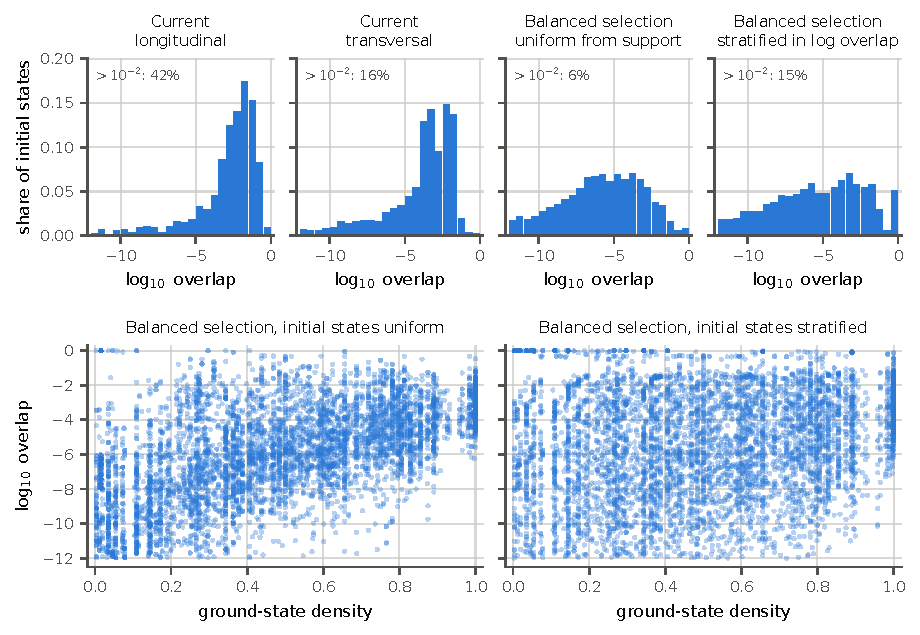
\includegraphics[width=\linewidth]{figures/overlap_comparison.pdf}
\caption{Top: overlaps of the initial states, six per kept Hamiltonian. Bottom: overlap
against ground-state density for the balanced selection. Each column of points is one
Hamiltonian. Dense ground states can only offer overlaps near $2^{-N}$.}
\label{fig:overlap}
\end{figure}

\paragraph{Smaller points.}
\begin{itemize}[leftmargin=1.2em]
\item The field is now two numbers. Add a facet for $\theta=\arctan(B_x/B_z)$ or for $B_x$ next to
  \texttt{Bz} in \texttt{FACETS}, otherwise the \texttt{Bz} folders mix very different fields.
\item 11\% of the selected Hamiltonians are near-product states (top weight $>0.99$), and the
  smallest gap is $3\times10^{-4}$, just above the cut. If either worries you, tighten
  \texttt{MIN\_GAP} or the trivial cut in \texttt{select\_hamiltonians.py} as well, so that the
  table and the plots agree.
\item The study here covers \texttt{max\_distance}~$=1$ and $B_y=0$, as in the current runs.
\end{itemize}

\paragraph{Reproducing.} In \texttt{StudyOfHamiltonians/}: \texttt{scan\_grid.py} (grid, Fig.~2),
\texttt{simulate\_schemes.py} (current and candidate draws), \texttt{select\_hamiltonians.py}
(balanced table), \texttt{make\_figures.py}, then \texttt{pdflatex report.tex}. Nothing outside
the folder is modified. \texttt{RandomSpinModel.py} is only imported.

\end{document}
